% generated by scripts/pkl_to_latex.py
% source PKL : thermal_v1_L6_Ne5_U10_t1_mode-uniform_tpall_t2all_tperpall_nmin2_solver-gcg_full_restarts10_iter300_kmax4_tol1em09_cut10_adaptive1_step5_clusteravg1_T0to5_N40-205b87919d2f_knone_diag0.pkl
% scan type  : Tscan
% state      : gs
% requires   : \usepackage{pgfplots} \pgfplotsset{compat=1.18}
% colours match the matplotlib PDF (tab10 cycle)
\definecolor{gmeC0}{HTML}{1F77B4}
\definecolor{gmeC1}{HTML}{FF7F0E}
\definecolor{gmeC2}{HTML}{2CA02C}
\definecolor{gmeC3}{HTML}{D62728}
\definecolor{gmeC4}{HTML}{9467BD}
\definecolor{gmeC5}{HTML}{8C564B}
\definecolor{gmeC6}{HTML}{E377C2}
\definecolor{gmeC7}{HTML}{17BECF}

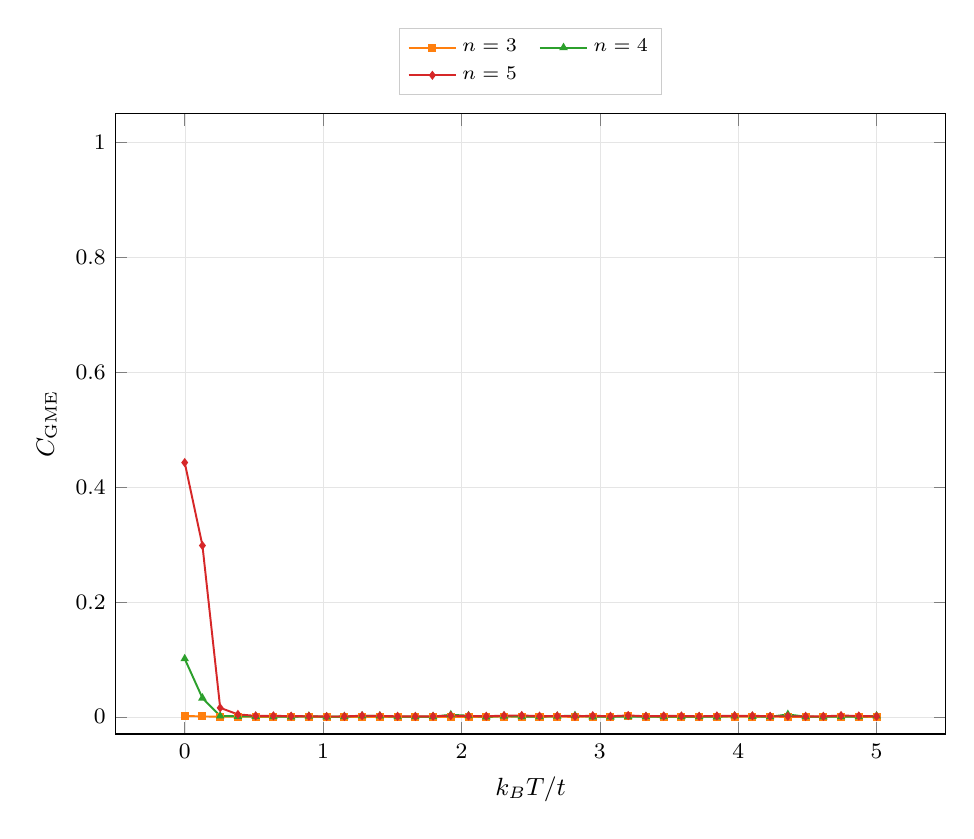
\begin{tikzpicture}
  \begin{axis}[
    width=\columnwidth,
    height=0.78\columnwidth,
    xlabel={$k_B T/t$},
    ylabel={$C_{\mathrm{GME}}$},
    grid=both,
    grid style={line width=.1pt, draw=gray!20},
    tick label style={font=\footnotesize\rmfamily, /pgf/number format/fixed},
    label style={font=\small\rmfamily},
    scaled ticks=false,
    legend style={font=\scriptsize\rmfamily, draw=gray!40, at={(0.5,1.03)}, anchor=south, /tikz/every even column/.append style={column sep=6pt}},
    legend cell align={left},
    legend columns=2,
    ymin=-0.03,
    ymax=1.05,
  ]
    \addplot[color=gmeC1, mark=square*, mark size=1.1pt, line width=0.7pt] coordinates {
        (0,0.001427) (0.128205,0.000719) (0.25641,0.000063) (0.384615,0.000198)
        (0.512821,0.000038) (0.641026,0.000038) (0.769231,0.000466) (0.897436,0.00006)
        (1.025641,0.000001) (1.153846,0.000044) (1.282051,0.000034) (1.410256,0.000015)
        (1.538462,0.000003) (1.666667,0.000039) (1.794872,0.000026) (1.923077,0)
        (2.051282,0.000004) (2.179487,0.000001) (2.307692,0.000124) (2.435897,0.000236)
        (2.564103,0.000014) (2.692308,0.000102) (2.820513,0.000007) (2.948718,0.000155)
        (3.076923,0.000007) (3.205128,0.001695) (3.333333,0.000103) (3.461538,0.000013)
        (3.589744,0.000004) (3.717949,0.000021) (3.846154,0.000415) (3.974359,0.000318)
        (4.102564,0.000004) (4.230769,0.000099) (4.358974,0) (4.487179,0.000005)
        (4.615385,0.000001) (4.74359,0.000192) (4.871795,0.000001) (5,0)
    };
    \addlegendentry{$n=3$}
    \addplot[color=gmeC2, mark=triangle*, mark size=1.1pt, line width=0.7pt] coordinates {
        (0,0.101118) (0.128205,0.032668) (0.25641,0.001425) (0.384615,0.000895)
        (0.512821,0.000886) (0.641026,0.000399) (0.769231,0.000022) (0.897436,0.001141)
        (1.025641,0.00007) (1.153846,0.00052) (1.282051,0.001557) (1.410256,0.001615)
        (1.538462,0.000176) (1.666667,0.000193) (1.794872,0.000389) (1.923077,0.003465)
        (2.051282,0.001929) (2.179487,0.000025) (2.307692,0.001357) (2.435897,0.000238)
        (2.564103,0.000279) (2.692308,0.001053) (2.820513,0.0021) (2.948718,0.000074)
        (3.076923,0.000076) (3.205128,0.000274) (3.333333,0.000322) (3.461538,0.000101)
        (3.589744,0.000351) (3.717949,0.000378) (3.846154,0.000038) (3.974359,0.001484)
        (4.102564,0.00081) (4.230769,0.000125) (4.358974,0.004063) (4.487179,0.000267)
        (4.615385,0.000033) (4.74359,0.000131) (4.871795,0.000187) (5,0.001664)
    };
    \addlegendentry{$n=4$}
    \addplot[color=gmeC3, mark=diamond*, mark size=1.1pt, line width=0.7pt] coordinates {
        (0,0.442751) (0.128205,0.298246) (0.25641,0.015621) (0.384615,0.004185)
        (0.512821,0.00163) (0.641026,0.001746) (0.769231,0.00111) (0.897436,0.000982)
        (1.025641,0.000518) (1.153846,0.000627) (1.282051,0.001965) (1.410256,0.001604)
        (1.538462,0.000818) (1.666667,0.000679) (1.794872,0.00086) (1.923077,0.002009)
        (2.051282,0.001395) (2.179487,0.000937) (2.307692,0.002103) (2.435897,0.00235)
        (2.564103,0.001142) (2.692308,0.001571) (2.820513,0.000829) (2.948718,0.001911)
        (3.076923,0.000905) (3.205128,0.00238) (3.333333,0.000964) (3.461538,0.001515)
        (3.589744,0.001507) (3.717949,0.000821) (3.846154,0.001597) (3.974359,0.001639)
        (4.102564,0.001806) (4.230769,0.000919) (4.358974,0.000919) (4.487179,0.000792)
        (4.615385,0.000866) (4.74359,0.002211) (4.871795,0.001499) (5,0.000758)
    };
    \addlegendentry{$n=5$}
  \end{axis}
\end{tikzpicture}
